\begin{refsection}
\chapter{The context dependency of pollinator interference: how environmental conditions and co-foraging species impact floral visitation} % Main chapter title
\label{Bee_foraging}

\noindent Alba Cervantes-Loreto\textsuperscript{1}, Carolyn A.\ Ayers \textsuperscript{2}, Emily K.\ Dobbs\textsuperscript{2},Berry J.\ Brosi\textsuperscript{3}, Daniel B.\ So\textsuperscript{1}

\begin{enumerate}
    \item Centre for Integrative Ecology, School of Biological Sciences, University of Canterbury, New Zealand
    \item Department of Environmental Sciences, Emory University, Atlanta, Georgia USA
    \item University of Washington, Department of Biology, Seattle USA
\end{enumerate}

\section*{Abstract}
Animals often change their behavior in the presence of other species and the environmental context they experience, and these changes can substantially modify the course their populations follow. In the case of animals involved in mutualistic interactions, it is still unclear how to incorporate the effects of these behavioral changes into population dynamics. We propose a framework for using pollinator functional responses to examine the roles of pollinator--pollinator interactions and abiotic conditions in altering the times between floral visits of a focal pollinator. We then apply this framework to a unique foraging experiment with different models that allow resource availability and sub-lethal exposure to a neonicotinoid pesticide to modify how pollinators forage alone and with co-foragers. We found that all co-foragers interfere with the focal pollinator under at least one set of abiotic conditions; for most species, interference was strongest at higher levels of resource availability and with pesticide exposure. Overall our results highlight that density-dependent responses are often context-dependent themselves.

\section*{Introduction}
Interactions between pollinators have been extensively documented and described by ecologists \citep{mallinger2017managed, thomson_importance_2020}. For eusocial insects like some bees and bumblebees, the presence of other species has been shown to drive resource partitioning due to active avoidance \citep{morse_resource_1977, inouye_resource_1978}, change pollinator foraging efforts  \citep{thomson_detecting_2006}, and to promote short-term floral specialization \citep{brosi_single_2013, briggs_competitive_2016}. However, fundamental gaps remain regarding the consequences of pollinator--pollinator interactions in natural communities, mainly because of the complexity of linking the effects of the interaction to population dynamics \citep{thomson_importance_2020}.


One of the empirical challenges in understanding interactions between pollinators is that environmental conditions can drastically change how pollinators behave and interact with conspecifics and other species. For instance, plant--pollinator interactions tend to be contingent on the external conditions pollinators experience \citep{heinrich_resource_1976,cnaani_flower_2006}. High resource availability---measured in flower density or nectar volume---has been shown to decrease the duration of foraging trips for bumblebees \citep{westphal_foraging_2006} and increase floral visits \citep{thomson_response_1987, thomson_effects_1988}. Insect pollinators also show changes in their interactions with plants due to temperature; higher temperatures have been documented to shorten the time spent on individual flowers relative to low temperatures for bumblebees \citep{heinrich_energetics_1972} and to promote floral specialization within an elevation gradient \citep{classen2020specialization}. Hence, studying the context in which interactions occur is as important as studying the interactions themselves.


In contrast, a theoretical challenge is incorporating the behavioral changes driven by the presence of other foraging pollinators, henceforth co-foragers, into population dynamics. Pollinator functional responses, which describe how consumption rates vary with the abundance of individuals of another population \citep{holland_population_2001}, are key to how pollinator and plant populations are linked to each other. When pollinators modify their behavior due to the presence of other foraging species, it echoes observations in which predators' consumption rates vary because of ``interference'': time spent engaging in encounters with other predators instead of feeding \citep{beddington_mutual_1975,deangelis_emergence_2006,skalski_functional_2001}.

Overt interference between pollinators is thought to occur only for very specific groups of pollinators that present aggressive behavior, such as stingless bees that can recruit in large numbers and inflict serious damage to their competitors \citep{lichtenberg_olfactory_2011}. Nonetheless, the presence of other foragers could have the same phenomenological effect as overt interference---from a functional response perspective---as long as it decreases the visitation rates of a focal individual. Importantly, the presence of other pollinator species can also increase visitation rates \citep[e.g.][]{greenleaf_wild_2006}. Overall, whether or not the presence of other species leads to measurable differences in the rate of floral visits has equivocal experimental evidence: some studies report an increase in visits and pollination efficiency when more than one species is present \citep{frund_bee_2013} whereas others find an overall decrease in foraging activity \citep{roubik_competitive_1978, thomson_detecting_2006, thomson_importance_2020}. That the effect of varying pollinator abundances is context dependent could potentially explain the equivocal evidence found across the literature.


Fully incorporating pollinator behavioral changes into population dynamics is a laborious and challenging effort since it not only requires quantifying functional responses of the populations involved but the numerical responses as well \citep{revilla2015numerical, abrams_nature_2000}. Nonetheless, since interactions and vistation are a necessary precursor to a quantifiable numerical response, a good starting place is to determine how biotic and abiotic factors can be incorporated into pollinator's foraging rates. In this study, we therefore show how plant--pollinator functional responses can be used to incorporate the effects of environmental conditions and pollinator--pollinator interactions into floral visitation rates. We first introduce a novel framework that examines a simple response variable: the time a pollinator takes between floral visits. We then use our functional response framework to quantify the effects of pollinator--pollinator interactions under different environmental conditions in a highly controlled foraging-chamber experiment. Our experiments simultaneously modified varying levels of resource availability, sub-lethal exposure to a neonicotinoid pesticide, and co-foraging pollinator richness and abundance. We parameterize different models that incorporate pollinator--pollinator interactions and environmental conditions when predicting observed times between floral visits. Finally, we use these model fits to show that pollinator--pollinator interactions and their effects on focal pollinators are strongly determined by abiotic conditions.

\section*{Methods}

\subsection*{A functional response framework of times between floral visits}

To understand the effect of varying abundances of plants and pollinators, as well as different environmental conditions, we build upon a classical framework to quantify consumption rates in consumer--resource systems. First, to mathematically describe how frequently a focal individual from pollinator species $i$ visits flowers as floral abundance changes, we assumed the per capita visitation rate takes the form of a Type II functional response \citep{holling1959some} as this is the predominant form assumed in various studies employing functional responses for mutualists \citep{holland2002population, valdovinos_adaptive_2013, bastolla2009architecture, rohr_structural_2014}. Second, to describe how floral visits change with varying abundances of pollinators, we developed an analogue to the Beddington--DeAngelis functional response \citep{beddington_mutual_1975,deangelis_model_1975}. This function assumes that the instantaneous per capita flower visitation rate of a focal pollinator from species $i$ on focal flowers of the species $m$, $\lambda_{i,m}$, is a non-linear function with the form:
\begin{equation}
    \label{lambda}
	\lambda_{i,m}  = \frac{a_{m}N_{m}}{1+a_{m}h_{m}N_{m}+ \sum_{n}a_{n}h_{n}N_{n} +c_{i}(P_{i}-1) + \sum_{j}c_{j} P _{j}} \,,
\end{equation}
where $N_{m}$ and $N_{n}$ are the abundances of focal and non-focal flowers. The encounter rate of bee individuals with focal flowers is described by $a_{m}$, while $a_{n}$ describes the encounter rate with non-focal flowers. Similarly, $h_{m}$ and $h_{n}$ denote the handling times of focal and non-focal flowers, respectively. The variables $P_{i}$ and $P_{j}$ represent the conspecific and heterospecific pollinator abundances, respectively, and their effects on visitation are captured by $c_{i}$ and $c_{j}$. Note that for conspecific interactions between pollinators, we used $P_{i}-1$ to account for the fact that focal individuals do not interact with themselves.

Though they are rarely studied in this way due to the typical data available, an alternative and equivalent approach to characterize functional responses is to examine the time between feeding events instead of feeding rates themselves \citep{coblentz2020estimating}. This approach has the advantage of allowing inferrence of a consumer's functional response using one or a few trials per individual \citep{coblentz2020estimating}. Returning to the functional response given by Eq.~\ref{lambda}, we can estimate time between floral visits, $\rho_{i,m}$, as the inverse of the per capita visitation rate:
  \begin{equation}
    \label{rho}
	\rho_{i,m} =
	\frac{1}{\lambda_{i,m}} =
	\frac{1}{a_{m}N_{m}} +
	 h_{m} +
	 \frac{1}{a_{m}N_{m}}\sum_{n}a_{n}h_{n}N_{n}+
	 \frac{c_{i}}{a_{m}N_{m}} (P_{i}-1)+
	 \frac{1}{a_{m}N_{m}} \sum_{j} c_{j}P_{j}  \text{.}
  \end{equation}
Written this way, the times between floral visits become the sum of the time each focal pollinator spends between visiting focal flowers, the time between visiting other flowers, and the time ``added'' by interactions with conspecific and heterospecific co-foragers. Importantly, the effects of pollinator--pollinator interactions can be quantified as increases or decreases to the times between floral visits. Note that conversion of times between visits to visitation rates can be done for either when the number of flowers or the number of pollinator vary (Fig.~\ref{fig:fig1}).


\begin{figure}[H]
    \centerline{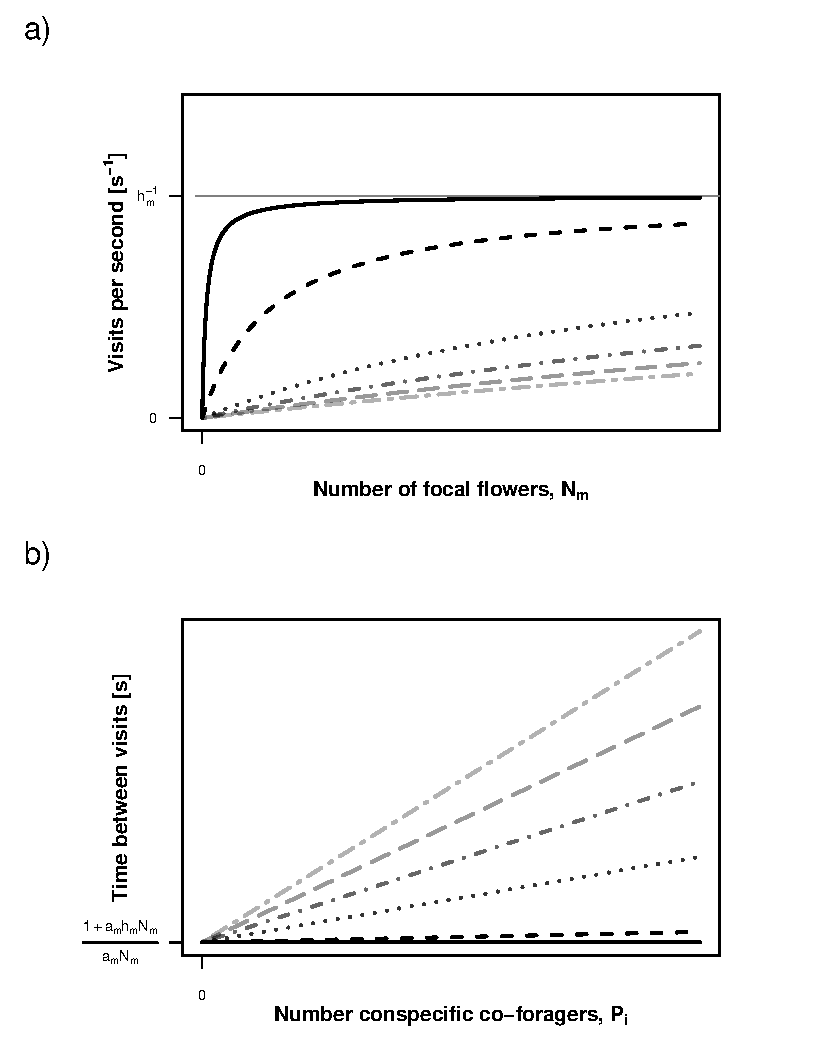
\includegraphics[height=0.7\textheight]{figures/chapter2_fig1.pdf}}
    \caption[Visualizing the mathematical relationship between visitation rate and time between visits.]{Visualizing the mathematical relationship between visitation rate and time between visits. a) Visitation rate as a function of the number of flowers $N_{m}$ (Eq~.\ref{lambda}). For a fixed number of co-foraging conspecific pollinators $P_{i}$ with no interference ($c_{i}$ = 0), no heterospecific pollinators present ($P_{j}$ = 0), and no other plants ($N_{n}$ = 0), the visitation rate saturates at at 1/$h_{m}$ (solid black line). As $c_{i}$ increases (dashed and dotted lines in lighter colours), the rate at which visitation rate reaches saturation decreases. b) Time between visits to a fixed number of focal flowers $N_{m}$ as a function of conspecific co-foragers $P_{i}$, also with $P_{j}$ = 0 and $N_{n}$ = 0 (Eq~.\ref{rho}). When $c_{i}$ = 0, the time between floral visits does not change with increasing pollinator abundance (solid black line). As $c_{i}$ increases, each co-foraging pollinator contributes more time to the time between floral visits (dashed and dotted lines in lighter colours as in a). }
    \label{fig:fig1}
\end{figure}

This general functional response framework allows us to quantify visitation rates under several experimental designs that might include scenarios (i) where floral abundances vary, (ii) where pollinator abundances vary, and (iii) under different environmental conditions.
For example, when there are observations of a focal pollinator and conspecific co-foragers visiting varying abundances of two plants, Eq.~\ref{rho} reduces to:
\begin{equation}
	\label{single_pollinator}
\rho_{i,m} = \frac{1}{a_{m}N_{m}}+ h_{m} + \frac{a_{n}h_{n}N_{n}}{a_{m}N_{m}} +\frac{c_{i}}{a_{m}N_{m}} (P_{i}-1)  \text{.}
\end{equation}

Note that to parameterize Eq.~\ref{single_pollinator}, we require independent variations of the abundances of both flowers \textit{and} of pollinators. However, it is also possible to adapt and fit a model based on our framework when only \emph{some} abundances change. For instance, if  the number of conspecific co-foragers $P_i$ is fixed, Eq.~\ref{single_pollinator} becomes:
\begin{equation}
	\label{single_pollinator_simple}
\rho_{i,m} =  h_{m} + \left ( \frac{1}{a_{m}} + \frac{c_{i}(P_{i}-1)}{a_{m}}\right ) \frac{1}{N_{m}} +  \left ( \frac{a_{n}h_{n}}{a_{m}}  \right ) N_{n} \frac{1}{N_{m}}
\end{equation}
which can be further simplified to:
\begin{equation}
	\rho_{i,m} = h_{m} + \gamma_{i,m} \frac{1}{N_{m}} + \delta_{i,n} N_{n} \frac{1}{N_{m}}  \text{.}
\end{equation}
Here the composite parameter $\gamma_{i,m}$ scales the impact of changes in focal floral abundances in the time between floral visits while $\delta_{i,m}$ scales the relative impact of changes in non-focal floral abundances. Since $\gamma_{i,m}$ includes encounter rates with flowers as well as the implicit impact of pollinator interference, these cannot be disentangled statistically without variation in $P_{i}$. Similarly, $\delta_{i,m}$ is a term that includes both the encounter rates with focal and with non-focal flowers.

On the other hand, when there are observations of different abundances of co-foragers visiting a fixed number of flowers of a single species, then Eq.~\ref{rho} becomes:
\begin{equation}
	\label{multiple_coforagers}
\rho_{i,m} = \frac{1+a_{m}h_{m}N_{m}}{a_{m}N_{m}} +\frac{c_{i}}{a_{m}N_{m}} (P_{i}-1) +\frac{c_{j}}{a_{m}N_{m}} P_{j}  \text{,}
\end{equation}
which can be further simplified to:
\begin{equation}
\label{interference_2}
		\rho_{i,m} =\alpha_{m} + \beta_{i,m} (P_{i}-1) + \beta_{j,m} P_{j} \,,
\end{equation}
where the composite parameter $\alpha_{m}$ sets a baseline of time between visits when there are no pollinator--pollinator interactions (i.e.\ the pollinator density-independent foraging outcomes), and the composite parameters $\beta_{i,m}$ and $\beta_{j,m}$ capture the  density-dependent changes to the time between visits to focal flowers. As above, both $\beta_{i,m}$ and $\beta_{j,m}$ incorporate both pollinator interference and encounter rates with flowers. Thus, an increase of times between floral visits (i.e.\ a decrease in floral visitation rates) could be the outcome of higher pollinator interference or decreasing encounter rates with flowers.

As a final example, both the density-dependent and density-independent terms can be inferred under different environmental conditions. For example, suppose we measure an enviomental variable $E$, and there are observations similar to those of Eq.~\ref{multiple_coforagers} but under different levels of the enviomental condition. Then, Eq.~\ref{interference_2} can be expanded into:
\begin{equation}
\label{interference_environment}
		\rho_{i,m} =\alpha_{m}+
		\alpha_{m,e} E +
	   (\beta_{i,m} + \beta_{i,m,e} E) (P_{i}-1) +
		(\beta_{j,m} + \beta_{j,m,e} E ) P_{j} \,,
\end{equation}
where $E$ is the value of the measured environmental variable (which can take continuous or discrete values), and the parameters with the subscript $e$ capture changes driven by abiotic conditions. For example, if $\beta_{i,m}$ quantifies the effect of conspecific pollinators, then $\beta_{i,m,e}$  quantifies how much the effect of conspecific pollinators changes under a certain abiotic condition. Written this way, both pollinator abundances and the enviomental conditions are the factors that determine the effect of pollinator--pollinator interactions.


\subsection*{Data}

In the following sections, we use our framework to parameterize and compare different models of floral visits with a unique foraging experiment. To do so, we examined data from a set of experiments that allowed us to tightly monitor the time  individual bumblebees spend between visits to artificial flowers, as well as the energy consumed per visit. During 2015 and 2016, we tracked the activity of commercial \textit{Bombus impatiens} (henceforth \textit{Bombus}) from Koppert Biological Systems (Howell, MI USA), inside a foraging chamber under (i) different richness and abundances of co-foragers and (ii) different levels of resource availability (iii) with and without pesticide exposure. These data  belong the ``Emory data set'', as described in \citet{ayers_statistically_2018}.

\subsubsection*{Experimental setup}

To monitor the activity of our focal species, our enclosure consisted of an array of artificial flowers that recorded the presence of a visiting bee an at the same time dispensed an automatic computer-controlled reward. The system was made up of 32 artificial flowers in four rows of eight flowers each distributed uniformly inside the chamber. The artificial flowers varied by color (blue, white, yellow, pink), scent, and sucrose concentrations (2.0 M, 1.5 M, 1.0 M, 0.5 M), in a way that yielded four distinct flower types. The automatic tracking of \textit{Bombus} individuals and co-foragers was done using mic3-TAG RFID 16 kbit tags (Microsensys GmbH, Erfurt, Germany) attached to each bee's thorax so as to not interfere with movement of flight.

Corresponding RFID tag readers embedded in each artificial flower recorded the presence of a bee (of any species) and activated an automatic reward of  10 $\mu$l unless the same individual had been recorded in that flower in the last 30 seconds, in which case no reward was conferred. If a different individual, of any species, visited the same flower, then the granting of a new reward depended on the floral refill time, or the time after which artificial flowers would dispense a new sucrose reward after a previous visit, a condition that we manipulated throughout the trials (see \textit{Foraging trials}). The sucrose reward was dispensed from a pipette tip embedded in the artificial flower, which was taken up by the bee’s proboscis through capillary action. Data suggests that the bees were almost always consuming the full reward offered by the artificial flowers (Fig.~\ref{fig:flower_type} in \autoref{appendix_A}). This system allowed us to closely monitor the time between floral visits and energy consumption at the individual-bee level as well as resource availability using Arduino MEGA 2560 R3 hardware (Arduino LLC) and Processing software.


\subsubsection*{Foraging trials}

Foraging trials consisted of fasting the bees for one hour, transferring them to the foraging enclosure, and recording their behavior over 75 minutes. Before the experimental trials, we kept bees in separate training enclosures with artificial flowers identical to the ones in the experiment, except for the fact that training flowers were not computer controlled but delivered rewards \textit{ad libitum}. We simultaneously manipulated the richness and abundance of co-foragers, floral refill time, and the sub-lethal exposure to a common dose of a neonicotinoid pesticide as follows.

We manipulated the richness and abundance of co-foragers through a series of single-species and multi-species trials. In single-species trials, we varied the abundance of \textit{Bombus} to 4, 8 and 16 individuals foraging at the same time, with no other species present. In multi-species trials, we manipulated richness, or the number of species that were foraging at the same time as \textit{Bombus}. We examined the combinations of one to three additional bee species foraging at the same time as \textit{Bombus} while at all times holding total bee abundance constant at 16 individual bees. The three other species were another social bee species, \textit{Apis mellifera} (henceforth \textit{Apis}), and two solitary taxa, \textit{Osmia lignaria} and \textit{Megachile rotundata} (henceforth \textit{Osmia} and \textit{Megachile}). In multi-species trials, we used 8 \textit{Bombus} individuals for 2-species trials, either 5 or 6 \textit{Bombus} for 3-species trials, and 4 \textit{Bombus} for 4-species trials. We present a detailed description of the abundances of the other species during the experiment in Table \ref{tab:energy} in \autoref{appendix_A}.

We also manipulated floral refill time to mimic different levels of resource availability since resource availability for the foraging bees decreases as refill time increases. The levels of floral refill time we examined were: instantaneous refill (0 seconds), intermediate refill (120 seconds), and delayed refill (540 seconds). We will refer to instantaneous refill (i.e.\ high resource availability) as the control condition.

Finally, we also manipulated bee exposure to a sub-lethal dose of neonicotinoid pesticide. While in the training enclosure, we fed individuals of all species subject to the pesticide treatment \textit{ad libitum} on a sucrose solution with a sub-lethal concentration of 10 $\mu$g/L of thiamethoxam ($C_{8}H_{10}CIN_{5}O_{3}S$, Sigma Aldrich); bees subject to the control condition were fed a sucrose solution without pesticide. For bees subject to pesticide treatment, the solution that contained pesticide was their only available sugar source. Thiamethoxam is applied to a wide range of crops \citep{maienfisch_chemistry_2001} and the concentration is consistent to what insects experience in the field \citep{blacquiere_neonicotinoids_2012}. We ran trials with either all exposed (of all species) or all unexposed bees to mimic exposure at the landscape level. We show a detailed description of the number of trials and replicates we performed in Tables \ref{tab:si} and \ref{tab:mu} in \autoref{appendix_A}, as well as an explicit account of how the data was cleaned for analysis.

\subsection*{Analysis}

\subsubsection*{Models of times between floral visits}

Given our framework and our very detailed data-set, we were able to contrast different hypotheses regarding how pollinators forage and interact, using \textit{Bombus} as our focal species. Instead of testing \textit{all} possible hypotheses of how co-foragers, resouce availability and pesticide exposure influence the times between floral visits, we tested three relatively simple hypotheses: (i) \textit{Bombus} individuals forage unaffected by the presence of co-foragers or by environmental conditions, (ii) only co-foragers modify how \textit{Bombus} forages but environmental conditions do not, and (iii) environmental conditions modify how individuals forage alone and in the presence of other foragers. Our modelling aim was not to get a detailed prediction of the dynamics governing the experimental system, but rather to show that the modelled principles are sufficient to explain times between floral visits, following a demonstration modelling approach to reveal potential explanatory generalities \citep{evans2013simple}.


If we map our functional response framework to our experimental setup, we can describe the functional response of the focal \textit{Bombus} individuals with Eq.~\ref{interference_2}. Our hypotheses can then be tested across different foraging models that equate to further extensions or simplifications of Eq.~\ref{interference_2}. If the presence of co-foragers and environmental conditions have no effect on the times between visits across experiments, then a density-independent rate will be sufficient to describe the data:
 %
\begin{equation}
    \rho_{i}= \alpha \,.
    \label{null}
\end{equation}
 %
We call this our \textit{null} model. Note that since in our experiment floral abundances remained constant, we did not explore how changes in densities of different flower types changed foraging rates. Rather, we modelled how long \textit{Bombus} individuals would take between visits to all of the artificial flowers, regardless of the type of flower. Thus, for simplicity we dropped subscripts on terms that depended on flower types.

On the other hand, if co-foragers interact with each other but visitation is unaffected by the abiotic conditions, then an equation similar to Eq.~\ref{interference_2} that only considers the effect of co-foragers would best describe the times between floral visits. We call this the \textit{interference} model:
\begin{equation}
\label{interference_3}
		\rho_{i} =\alpha + \beta_{i} (P_{i}-1) + \sum_{j}\beta_{j}P_{j} \,.
\end{equation}

Finally, if the abiotic treatments modify how \textit{Bombus} forages with and without co-foragers, similiar to Eq.~\ref{interference_environment}, we would expect the times between visits to be a function of the abundance of co-foragers, level of resource availability ($R$) and pesticide exposure ($E$), we call this the \textit{treatments} model:
\begin{equation}
\begin{aligned}
\rho_{i} =\alpha + \alpha_{r} R+   \alpha_{e}E +  \beta_{i} (P_{i}-1) +  \beta_{i,r} (P_{i}-1) R +  \beta_{i,e} (P_{i}-1) E  \\      + \sum_{j}\beta_{j}P_{j}  +  \sum_{j}\beta_{j,r}P_{j}R +  \sum_{j}\beta_{j,e}P_{j}  E \,.
\end{aligned}
\label{treatments}
\end{equation}
Here the subscripts  $r$ and $e$ denote the parameters that estimate the effect of $R$ and $E$, respectively. In our case, $R$ is a continuous variable that corresponds to the floral refill time (i.e.\ goes from 0 to 540 seconds) and $E$ is a dummy variable to indicate pesticide exposure (i.e.\ $E = 0$ when bees are subject to the control treatment, and $E=1$ when bees were exposed to the pesticide treatment). The subscripts we used are consistent with the nomenclature of the density-independent and density-dependent terms described previously. Note that in our data, not all co-foraging species were tested under all experimental conditions (Table \ref{tab:mu} in \autoref{appendix_A}). Therefore, we did not model the three-way interaction between species identity, pesticide exposure and resource availability.


\subsubsection*{Statistical analyisis}

To  infer the parameters of Eqs.~(\ref{null}-\ref{treatments}), we fit non-linear hierarchical models with a Bayesian framework using Hamiltonian Monte Carlo (HMC) methods. We provide the details of our statistical analyisis in \autoref{appendix_A}. We fit our  models using the function  \textit{brm} from the package \textit{brms} \citep{burkner_advanced_2017} in the statistical program \textsc{R} (version 3.4.2) \citep{Rcore}. We ran four chains with a warm up of 3000 iterations and 2000 sampling iterations, using weakly informative priors and a maximum treedepth of 13 and an adapt delta of $0.99$. We determined convergence when trace plots were well mixed and stationary and when the Gelman-Rubin convergence diagnostic (Rhat) was less than 1.05 for all parameters \citep{vehtari_rank-normalization_2020}.

We compared the fits of  Eqs.~(\ref{null}-\ref{treatments}) to each other using the the Wanatabe-Akaike information criterion (WAIC) to determine which of the hypotheses encoded within the models best predicts out of sample times between floral visits. WAIC provides a measure for model fit that is penalized for the number of model parameters, and the best fit model in terms of out of sample predictions is the one with the lowest WAIC value. Additionally, we calculated Akaike weights for each model, which can be  interpreted as an estimate of the probability that the model will make the best predictions of new data based on the the set of models considered. We did model comparisons using 500 samples from the posterior distribution, and we defined best-fit models as those with the lowest WAIC and an Akaike weight greater than 0.9 \citep{mcelreath_statistical_2018}.

\section*{Results}

Model comparison using Wanatabe-Akaike information criterion (WAIC) showed that the \textit{treatments} model was the best-fit model for explaining the data by a wide margin (Table~\ref{tab:waic}). The \textit{treatments} model had the lowest WAIC score and received all of the Akaike weight, which means it had the highest probability to make the best predictions of new data compared to the two other models considered. Model comparison therefore showed not only that co-foraging pollinator abundances systematically modified the times between floral visits, but also that resource availability and pesticide exposure modified how bumblebees foraged alone and with other species present.

\subsection*{Density-independent effects}

The parameters of the \textit{treatments} model allowed us to make predictions beyond the pollinator densities manipulated during the trials since it estimated density-independent effects as the intercept. Without any co-foragers present, predictions using the \textit{treatments} model confirmed that both low resource availability and sub-lethal exposure to pesticide increased the time between floral visits (Fig.~\ref{fig:fig2}). Predictions made at low resource availability and under pesticide exposure (Fig.~\ref{fig:fig2}d) showed that a bumblebee foraging alone would spend on average 90 seconds more between floral visits when compared to predictions made at high resource availability and under no pesticide exposure (Fig.~\ref{fig:fig2}a); this equates to a near doubling of the amount of time between floral visits. Consequently, over the course of a 75 minute experiment, an average bumblebee foraging alone would make 15 fewer floral visits if there was low resource availability and it had been exposed to pesticide.

\begin{table}[H]
\centering
\caption[Model comparison table]{Model comparison table. WAIC (Widely Applicable Information Criteria) penalizes models for parameters, and the lowest WAIC reflects the best-fit model. pWAIC is the effective number of parameters and provides information on how flexible each model is in fitting the sample. Akaike Weight for each model is an estimate of the probability that the model will make the best predictions of new data based on the the set of models considered.}
\label{tab:waic}
\begin{tabular*}{\textwidth}{l @{\extracolsep{\fill}} ccc}
\toprule
model        & WAIC     & pWAIC  & Akaike weight        \\ \midrule
\textit{treatments}   & 413322.5 & 2386.6 & 1.00  \\
\textit{interference} & 414462.5 &  2135.6 & < .002 \\
\textit{null}         & 416063.6 &  1769.6  & < .002\\ \bottomrule
\end{tabular*}
\end{table}

As shown in the intercepts of Fig.~\ref{fig:fig2}a and c, we also found that the time between floral visits decreased as resource availability increased (i.e.\ the time between floral refill decreased). Predictions made at high resource availability (0 seconds between floral refill) showed that an average bumblebee would make 7 more floral visits over the course of an experiment than it would at low resource availability (540 seconds between floral refill).

\textit{Density-dependent effects}

We found that the time between floral visits for a focal pollinator changed consistently as a function of the identity and abundance of the co-foragers (Fig.~\ref{fig:fig2}). All of the species examined could potentially interfere with a focal \textit{Bombus} individual by increasing the time between floral visits, but the extent of the interference effect depended on the environmental context bees experienced.

Under control conditions (i.e.\ no pesticide exposure and high resource availability), increasing abundances of \textit{Bombus}, \textit{Osmia}, and \textit{Megachile} all increased the times between visits (and therefore decreased the visitation rate) to a similar extent (Fig.~\ref{fig:fig2}a). However, \textit{Apis} had an opposite effect under control conditions as increasing its density \emph{decreased} the times between floral visits. Thus, when there was high resource abundance and no pesticide exposure three of the species (including conspecifics) had an interference effect. However, as environmental conditions changed, so did these interference effects. For example, increasing abundances of \textit{Apis} changed from decreasing times between visits to increasing them when there was either pesticide exposure or low resource availability (Fig.~\ref{fig:fig2}).



\begin{figure}[H]
    \centerline{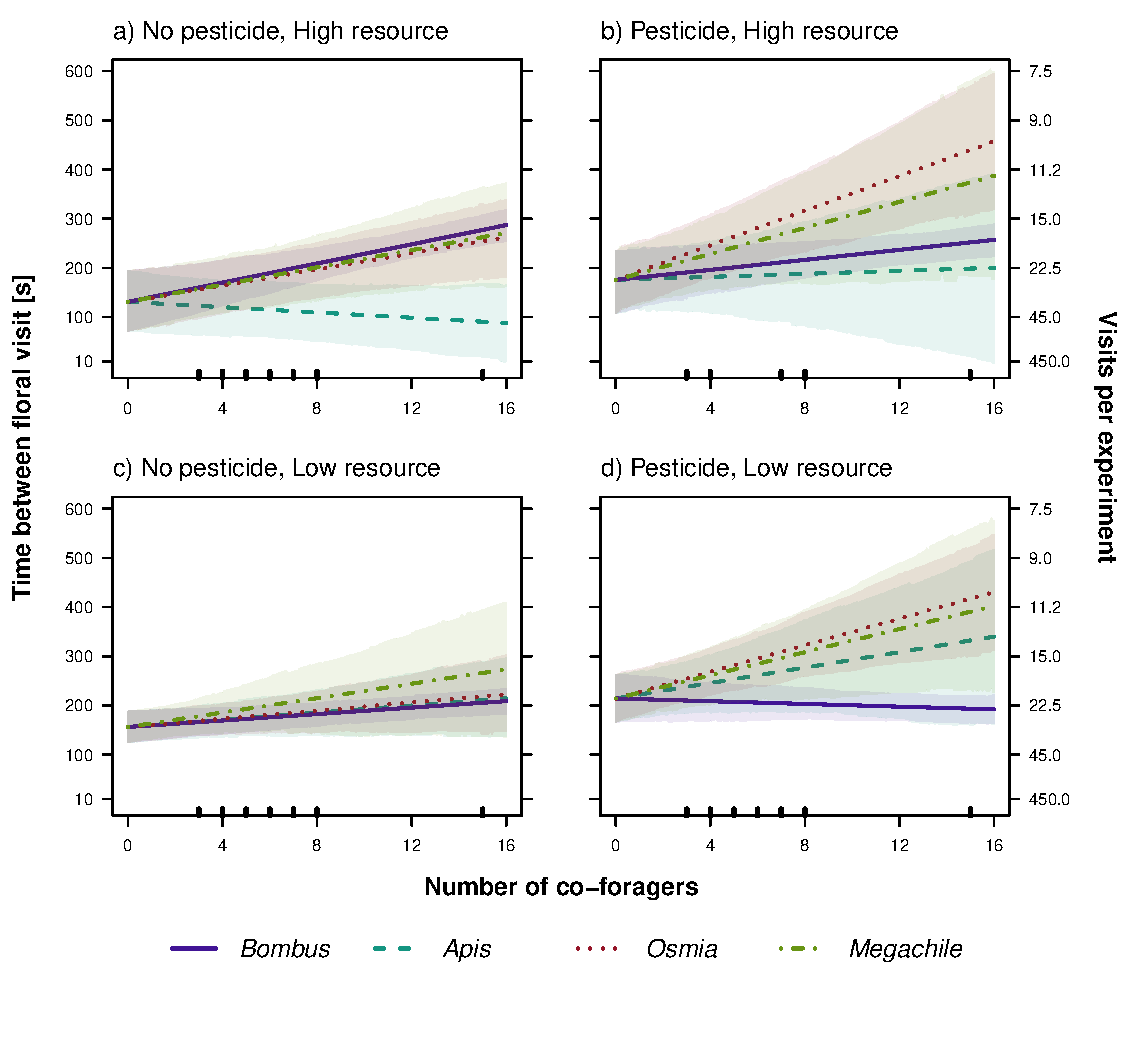
\includegraphics[height=0.7\textheight]{figures/chapter2_fig2.pdf}}
    \caption[Model predictions of how the time between floral visits changed as the number of co-foragers increased and under different environmental conditions]{ Model predictions of how the time between floral visits changed as the number of co-foragers increased and under different environmental conditions. Each color and line type correspond to a different co-forager. Lines represent predictions using the median parameter values of the \textit{treatments} model for the average focal individual. The shaded areas correspond to the 90\% highest posterior density interval (HPDI). High resource availability corresponds to 0 seconds between floral refill, and low resource availability to 540 seconds between floral refill (the maximum used during the experiments). Ticks along the x-axis indicate the actual co-forager abundances examined during the experimental trials. On the right y-axis and to help interpretation, we show how many visits per 75 minute experiment would be expected for the corresponding times between floral visits.}
    \label{fig:fig2}
\end{figure}{}

To better disentangle the species-specific response of interference to environmental variables, we estimated the time contributed by a single co-forager individual of each species to the total times between floral visits as resource availability increased (Fig.~\ref{fig:fig3}) and with the exposure to a neonicotinoid pesticide (Fig.~\ref{fig:fig4}). That is, given the posterior distribution of the fixed effects, we calculated how total times between floral visits changed due to the contribution of a single individual of each species under different environmental conditions. Note that due to the inverse relationship between time between floral visits and resource availability, Fig.~\ref{fig:fig3} shows decreasing times between floral refill.

We found that, as resources became more abundant (or the time between floral refill decreased), interference by \textit{Bombus}, \textit{Osmia}, and \textit{Megachile} increased (Fig.~\ref{fig:fig3}). In particular, the time contributed by a conspecific individual almost tripled when resource availability changed from low to high (Fig.~\ref{fig:fig3}a). For the majority of the species examined, interference was strongest when there was high resource availability, and its effect weakened as resources became more scarce. In contrast, as resources became more abundant, the contribution of an additional individual of \textit{Apis} to the time between floral visits decreased. Indeed, our predictions using median parameter values showed that an individual of \textit{Apis} went from creating net decreases in visitation rate at low resource availability to creating net increases in visitation rate at high resource availability (Fig.~\ref{fig:fig3}b). However, the predictions using the 90\% highest posterior density interval (HPDI, or the narrowest interval containing the specified probability mass \citep{mcelreath_statistical_2018}) for \textit{Apis} included competitive and facilitative outcomes at all levels of resource availability. Thus, even though on average \textit{Apis} individuals had a facilitative effect as resources became more abundant, we predicted some competitive effects as well when making predictions using the full posterior distribution.

In contrast to resource availability, pesticide exposure tended to increase the strength of pollinator interference for all species except \textit{Bombus}(Fig.~\ref{fig:fig4}). That is, when all of the bees had been exposed to pesticide, increasing heterospecific abundances of pollinators generally decreased floral visitation rate because individuals contributed positively to the times between floral visits. Conspecifics, however, had the opposite effect: pesticide exposure decreased the strength of pollinator interference (Fig.~\ref{fig:fig4}).


\begin{figure}[H]
    \centerline{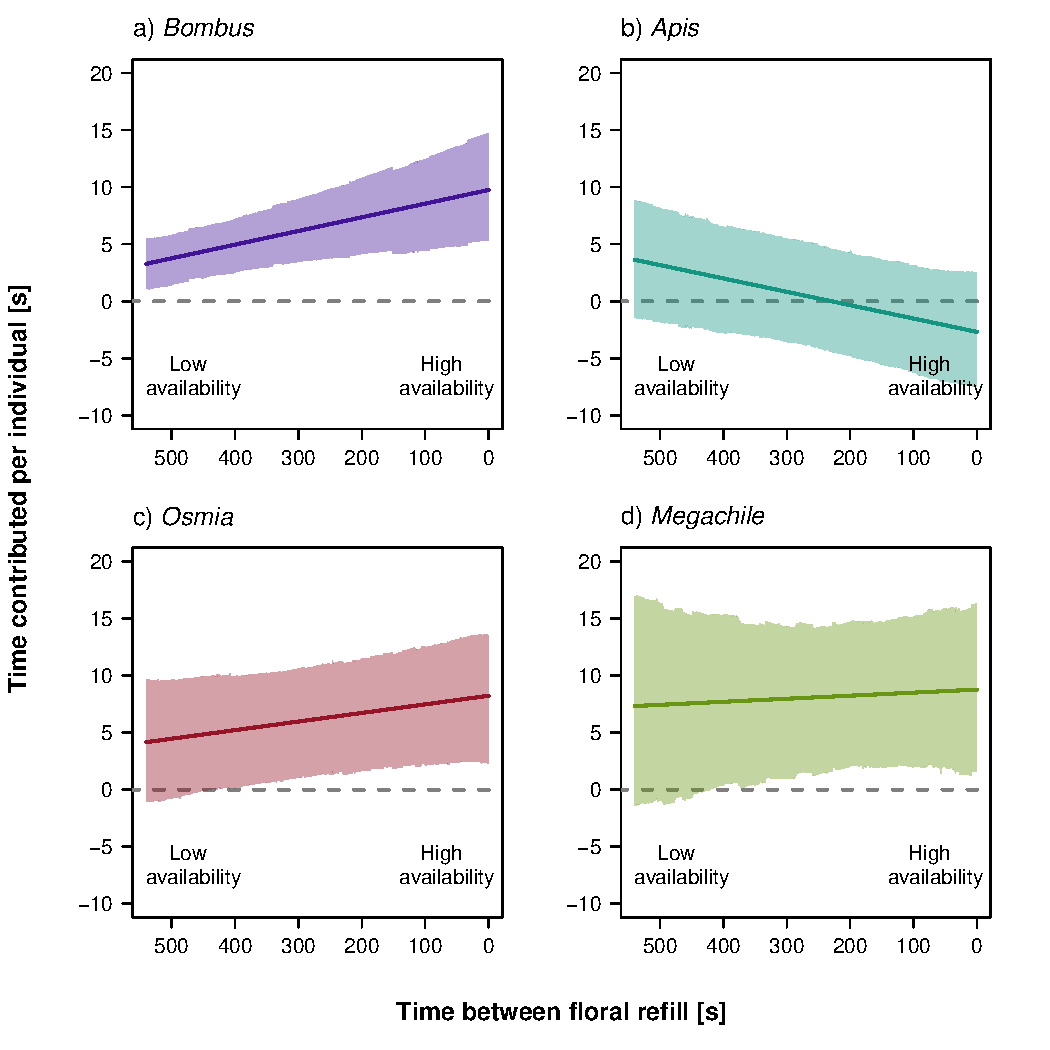
\includegraphics[height=0.7\textheight]{figures/chapter2_fig3.pdf}}
    \caption[Model predictions of the effect an individual co-forager had on the time between visits of \textit{Bombus} as resource availability increased]{Model predictions of the effect an individual co-forager had on the time between visits of \textit{Bombus} as resource availability increased and when there was no pesticide exposure. Each panel estimates the contribution of an individual co-forager from each of the four co-foraging species from our study. Solid lines represent the predictions made with the median parameter values of the \textit{treatments} model for the average focal individual whereas the shaded areas correspond to the 90\% highest posterior density interval (HPDI). To help interpretation, we provide the mapping between low and high resource availability and time between floral refill in each panel.  }
    \label{fig:fig3}
\end{figure}{}





\begin{figure}[H]
      \centerline{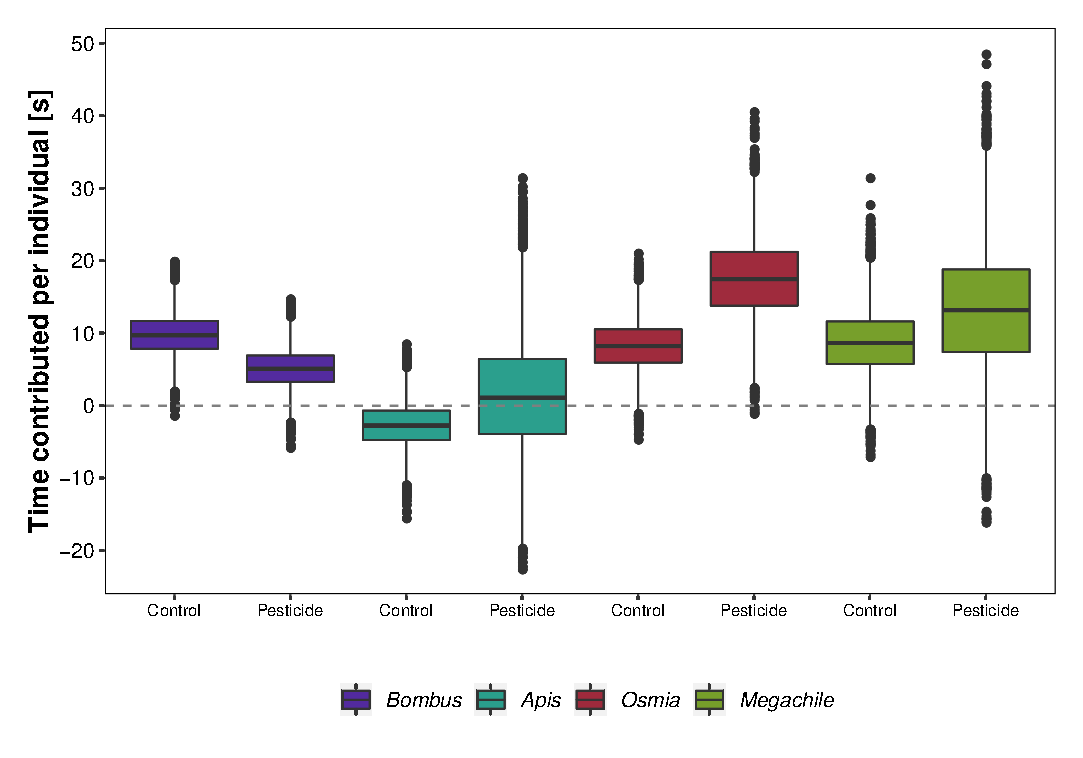
\includegraphics[width=1\textwidth]{figures/chapter2_fig4}}
    \caption[The effect an individual co-forager had on the time between floral visits]{ The effect an individual co-forager had on the time between floral visits when it had not been exposed to pesticide at high resource availability (Control), and when it had been exposed to a sub-lethal dose of neonicotinoid pesticide and at high resource availability (Pesticide). Each color corresponds to the different species of co-foragers. Each box plot extends from the first to third quantiles of the corresponding posterior distribution of parameter values, and the line inside the the box indicates the median. The upper whisker extends to the largest value no further than 1.5 times the inter-quantile range (IQR, or the distance between the first and third quartiles); the lower whisker extends to the smallest value at most 1.5 times the IQR. Data beyond the end of the whiskers are determined to be outliers and are plotted individually with solid black points.}
    \label{fig:fig4}
\end{figure}

\section*{Discussion}

%Paragraph to summarize the most important results that will be discussed below
We applied our functional response framework to illustrate how both environmental context and pollinator--pollinator interactions can substantially change the number of visits a pollinator will make. Our model predictions showed that when a pollinator was foraging alone, conditions such as low resource availability and exposure to a sub-lethal dose of pesticide decreased the visits made to flowers. However, the same environmental conditions could have opposite effects on pollinator--pollinator interactions; for most species examined, interference was strongest when there was high resource abundance, and pollinator interference decreased as resources became scarcer (except for \textit{Apis}). Finally, we found a density-dependent response to pesticide exposure since, for all co-foraging species except \textit{Bombus}, exposure to pesticide increased the sensitivity to individuals of other co-foraging species. On the whole, our results make clear that the question is not whether or not pollinators interfere with each other, but under what conditions they do so.


\subsection*{Resource abundance}

%The effects of resource abundance on a pollinator foraging alone
When resources are scarce, it has been previously documented that bumblebees make fewer visits to flowers than in rich-resource areas \citep{heinrich_bumblebee_2004,westphal_foraging_2006}. Our predictions agreed on the effect of low resource availability when a pollinator is foraging \textit{alone} (Fig.~\ref{fig:fig2}). For bumblebees, high resource availability can be associated with mass-flowering \citep{westphal_mass_2003}, and other studies have shown that net benefits are increased when bumblebees concentrate their efforts in areas of rich nectar resources while moving rapidly through depleted areas \citep{heinrich_resource_1979}.
%Thus, the increase in visitation rates with resource availability could be explained as a systematic exploitation of the most rewarding resources \citep{pyke_optimal_1978}.
%On the other hand, \citet{jha_resource_2013} found that bumblebees tend to increase visits in patches with high floral diversity, not density. Since the flower distribution (color, scent, and sucrose concentration) remained constant in our foraging chamber, we could only assess how resource abundance (measured in floral refill time) modifies foraging behavior.

%The effects of resource abundance on a pollinator foraging with other species
In contrast, the role of resources was reversed when a bumblebee foraged at the same time as other species. For most of the species examined, interference was strongest when resources were most abundant (Fig.~\ref{fig:fig3}). Recall that in our modeling framework an increase of times between floral visits can be caused by many different mechanisms. For example, we found with $\beta_{i,r}$ that the effect of conspecifics decreased as resources became more scarce. This decrease could be due to a decrease in overt interference, $c_{i}$, or to a lower encounter rates with flowers $a_{m}$. However, observations of bees during the experiments offer some potential insights into this question. First and foremost, we never observed obvious aggressive interactions between bee individuals in the foraging arena. Instead, interference appears to have been driven by avoidance of flowers due to visual and/or olfactory cues presented by other bee individuals. The response to these cues was clearly context dependent. For example, while we did not specifically test learning within individual bees, they may have learned within the course of a trial that a visual or olfactory cue of another individual at a flower signaled that the flower was unlikely to be rewarding (in the case of delayed floral refill) or that the cues were not related to rewards (in the case of instantaneous floral refill). Indeed, overt interference has not been observed in bumblebees \citep{heinrich_resource_1976, heinrich_bumblebee_2004}, but bumblebees have been documented to have avoidance behavior when foraging with other species \citep{morse_resource_1977, inouye_resource_1978} and  are able to detect and reject flowers which have been visited by other \textit{Bombus} species using scent \citep{goulson_foraging_1999}.

Additionally, different bee species behaved differently in the experiments and the contribution to the times between floral visits we found (positive and negative) was also reflective of competitor species identities. For example, \textit{Apis} individuals generated net increases in floral visits by decreasing the time between floral visits under high resource availability. This may be because honey bees were not particularly active in foraging and may have spent more time outside of flowers, which could have led to essentially an overall decrease in competition for \textit{Bombus}. Previous studies have found that interspecific interactions between honeybees and other species can sometimes result in an increase in pollination efficiency \citep{greenleaf_wild_2006}. In contrast, \textit{Megachile} individuals also had low foraging rates, but based on observations may have spent more time in and near flowers, potentially leading \textit{Bombus} individuals to avoid those flowers and increasing interference despite low foraging rates. Changes in bee foraging behavior have been shown to be species-specific before \citep{briggs_competitive_2016}, and it remains an exciting and open challenge to fully understand how they explicitly depend on environmental conditions.

% The effects of pesticide in general
\subsection*{Pesticide exposure}

Our results were also consistent with previous studies that saw a decrease in floral visits when pollinators are exposed to a sub-lethal dose of neonicotinoid pesticide \citep{gill_chronic_2014, henry_common_2012, stanley_chronic_2016, mommaerts_risk_2009}. Neonicotinoid pesticides bind strongly to nicotinic acetylcholine receptors in the central nervous system of insects \citep{goulson_review_2013}. At sub-lethal doses, this creates difficulties for memory and learning \citep{henry_common_2012}, as well as compromises navigation skills \citep{desneux_sublethal_2007}. Unsurprisingly, exposure to thiamethoxam increased the times between floral visits when a bumblebee was foraging alone and with the addition of individuals  of all of the heterospecific pollinators (Fig.~\ref{fig:fig2} \&\ref{fig:fig4}). For conspecifics, pesticide exposure weakened the effect of conspecific interference. That is, relative to the control conditions, foraging with conspecific individuals still resulted in a net decrease of floral visits but to a lesser extent. Thus, the general effect of sub-lethal exposure to a neonicotinoid pesticide is to decrease floral visits via both by density-dependent and density-independent mechanisms.

 %Given our experimental set-up, our results portray how we would expect bees to behave when all foraging species have been exposed to pesticide.

\subsection*{Experimental limitations }

In our study, the highly controlled experimental setup allowed us to tightly monitor bee behavior and thus explicitly quantify pollinator interference and its relationship with experimental treatments. However, the artificial environment  might not accurately capture how bees forage in the wild. For example, bumblebees could not leave low resource areas and concentrate their efforts in less depleted areas as they are prone to do \citep{heinrich_bumblebee_2004}. Furthermore, the non-focal species were not as active as \textit{Bombus} during the trials, which might further change how interference operates. Thus, the results presented here should be considered in the context of a controlled foraging experiment. This notwithstanding, we directly quantified behavioral changes driven by the presence of other pollinator species into pollinator functional responses, which has rarely been done.

\textit{Consequences of pollinator--pollinator interactions}

In this study we focused on the functional responses of pollinators, and did not quantify their numerical responses \citep{morris_benefit_2010}. Without knowing the numerical responses of the populations involved, we can not fully understand the dynamic consequences of pollinator--pollinator interactions \citep{revilla2015numerical}. However, our results do provide insights of how interference might affect mutualistic communities. Empirical and theoretical studies suggest that how often pollinators visit plants is a good predictor of the strength of the interaction, for both pollinators and plants involved \citep{vazquez_interaction_2005,vazquez_strength_2012}. Indeed, in our experimental system the number of floral visits was a good predictor of the energetic gains for bees, since bees seemed to almost always consume the full reward offered by artificial flowers (Fig~.\ref{fig:flower_type}, \autoref{appendix_A}). Thus, from the point of view of pollinators, foraging with other species can be disadvantageous under certain conditions. For example, if high resource abundance made the other species more active, \textit{Bombus} individuals might spend longer between flower visits because they are trying to avoid flowers that have already been visited. However, from the plant's perspective, receiving visits from a diverse pollinator assemblage can produce more stable plant reproduction \citep{sahli2006characterizing}, and greater competition tends to make bees increase floral fidelity, which also enchances plant fitness \citep{brosi_single_2013}. Much like plant diversity \citep{bruninga2016role}, our results show that pollinator diversity does not always have straightforward consequences on the populations involved.


\subsection*{Conclusion}

The impact of interactions between pollinators in natural communities it is still poorly understood. In this study, we argue that in order to understand when and why those interactions change the course of plant and pollinator populations, we should also determine the environmental context in which they occur. Importantly, our study provides a theoretical framework to do so, coupled with a highly controlled foraging experiment to show how drastically abiotic conditions can change the outcomes of pollinator--pollinator interactions. By incorporating intra-guild interactions into pollinator functional responses, our study opens up an urgent avenue to study the consequences of species loss and enviomental change in natural communities. It is critical to determine just how prevalent interference or facilitation between pollinator species is in nature, in order to further understand how species loss could affect pollinator populations. We believe our study gives ecologists the theoretical and statistical tools to quantify the effects of other species both in experimental and observational studies, and contributes to closing the gap between the mutualistic and predator--prey literatures.


%(Fig.~\ref{fig:fig1}).

\printbibliography
\end{refsection}
